\documentclass[12pt, a4paper]{article}
\usepackage[margin=1in]{geometry}
\usepackage{subfiles}
% document layout
% text options
\usepackage[T1]{fontenc}
\usepackage[spanish]{babel}

% headers and footers
\usepackage{fancyhdr}

% math extensions
\usepackage{amsmath}
\usepackage{siunitx}
\usepackage{physics}
\sisetup{per-mode=fraction}
\AtBeginDocument{\RenewCommandCopy\qty\SI}

% content layout
\usepackage{float}
\usepackage{booktabs}
\usepackage{subcaption}
\usepackage{adjustbox}
\usepackage{multirow}

% external imports
\usepackage{graphicx}

% references
\usepackage{hyperref}
\usepackage{csquotes}
\usepackage{biblatex}
\addbibresource{resources/references.bib}

%\AtBeginDocument{\RenewCommandCopy\qty\SI} %compiler's bug's patch

\begin{document}
\subfile{parts/cover}

% custon header and footer setup
\pagestyle{fancy}
\fancyfoot{} % clear all footer fields
\fancyfoot[L]{Facultad de Ciencias - UNI}
\fancyfoot[R]{\thepage}

\tableofcontents
\clearpage

\section{Objetivos}
\subfile{parts/objectives}

\section{Marco teórico}
\subfile{parts/theory}

\section{Equipo utilizado}
\subfile{parts/equipment}

\section{Procedimientos}
\subfile{parts/procedures}

\section{Tablas de datos}
\subfile{parts/tables}

\section{Cálculos y resultados}
\subfile{parts/results}

\section{Discusiones}
\subfile{parts/discussion}

\section{Conclusiones}
\subfile{parts/conclusion}

\section{Bibliografía}
\printbibliography

\clearpage

\listoffigures
\listoftables

\clearpage

\section{Anexo}
\begin{figure}[H]
    \centering
    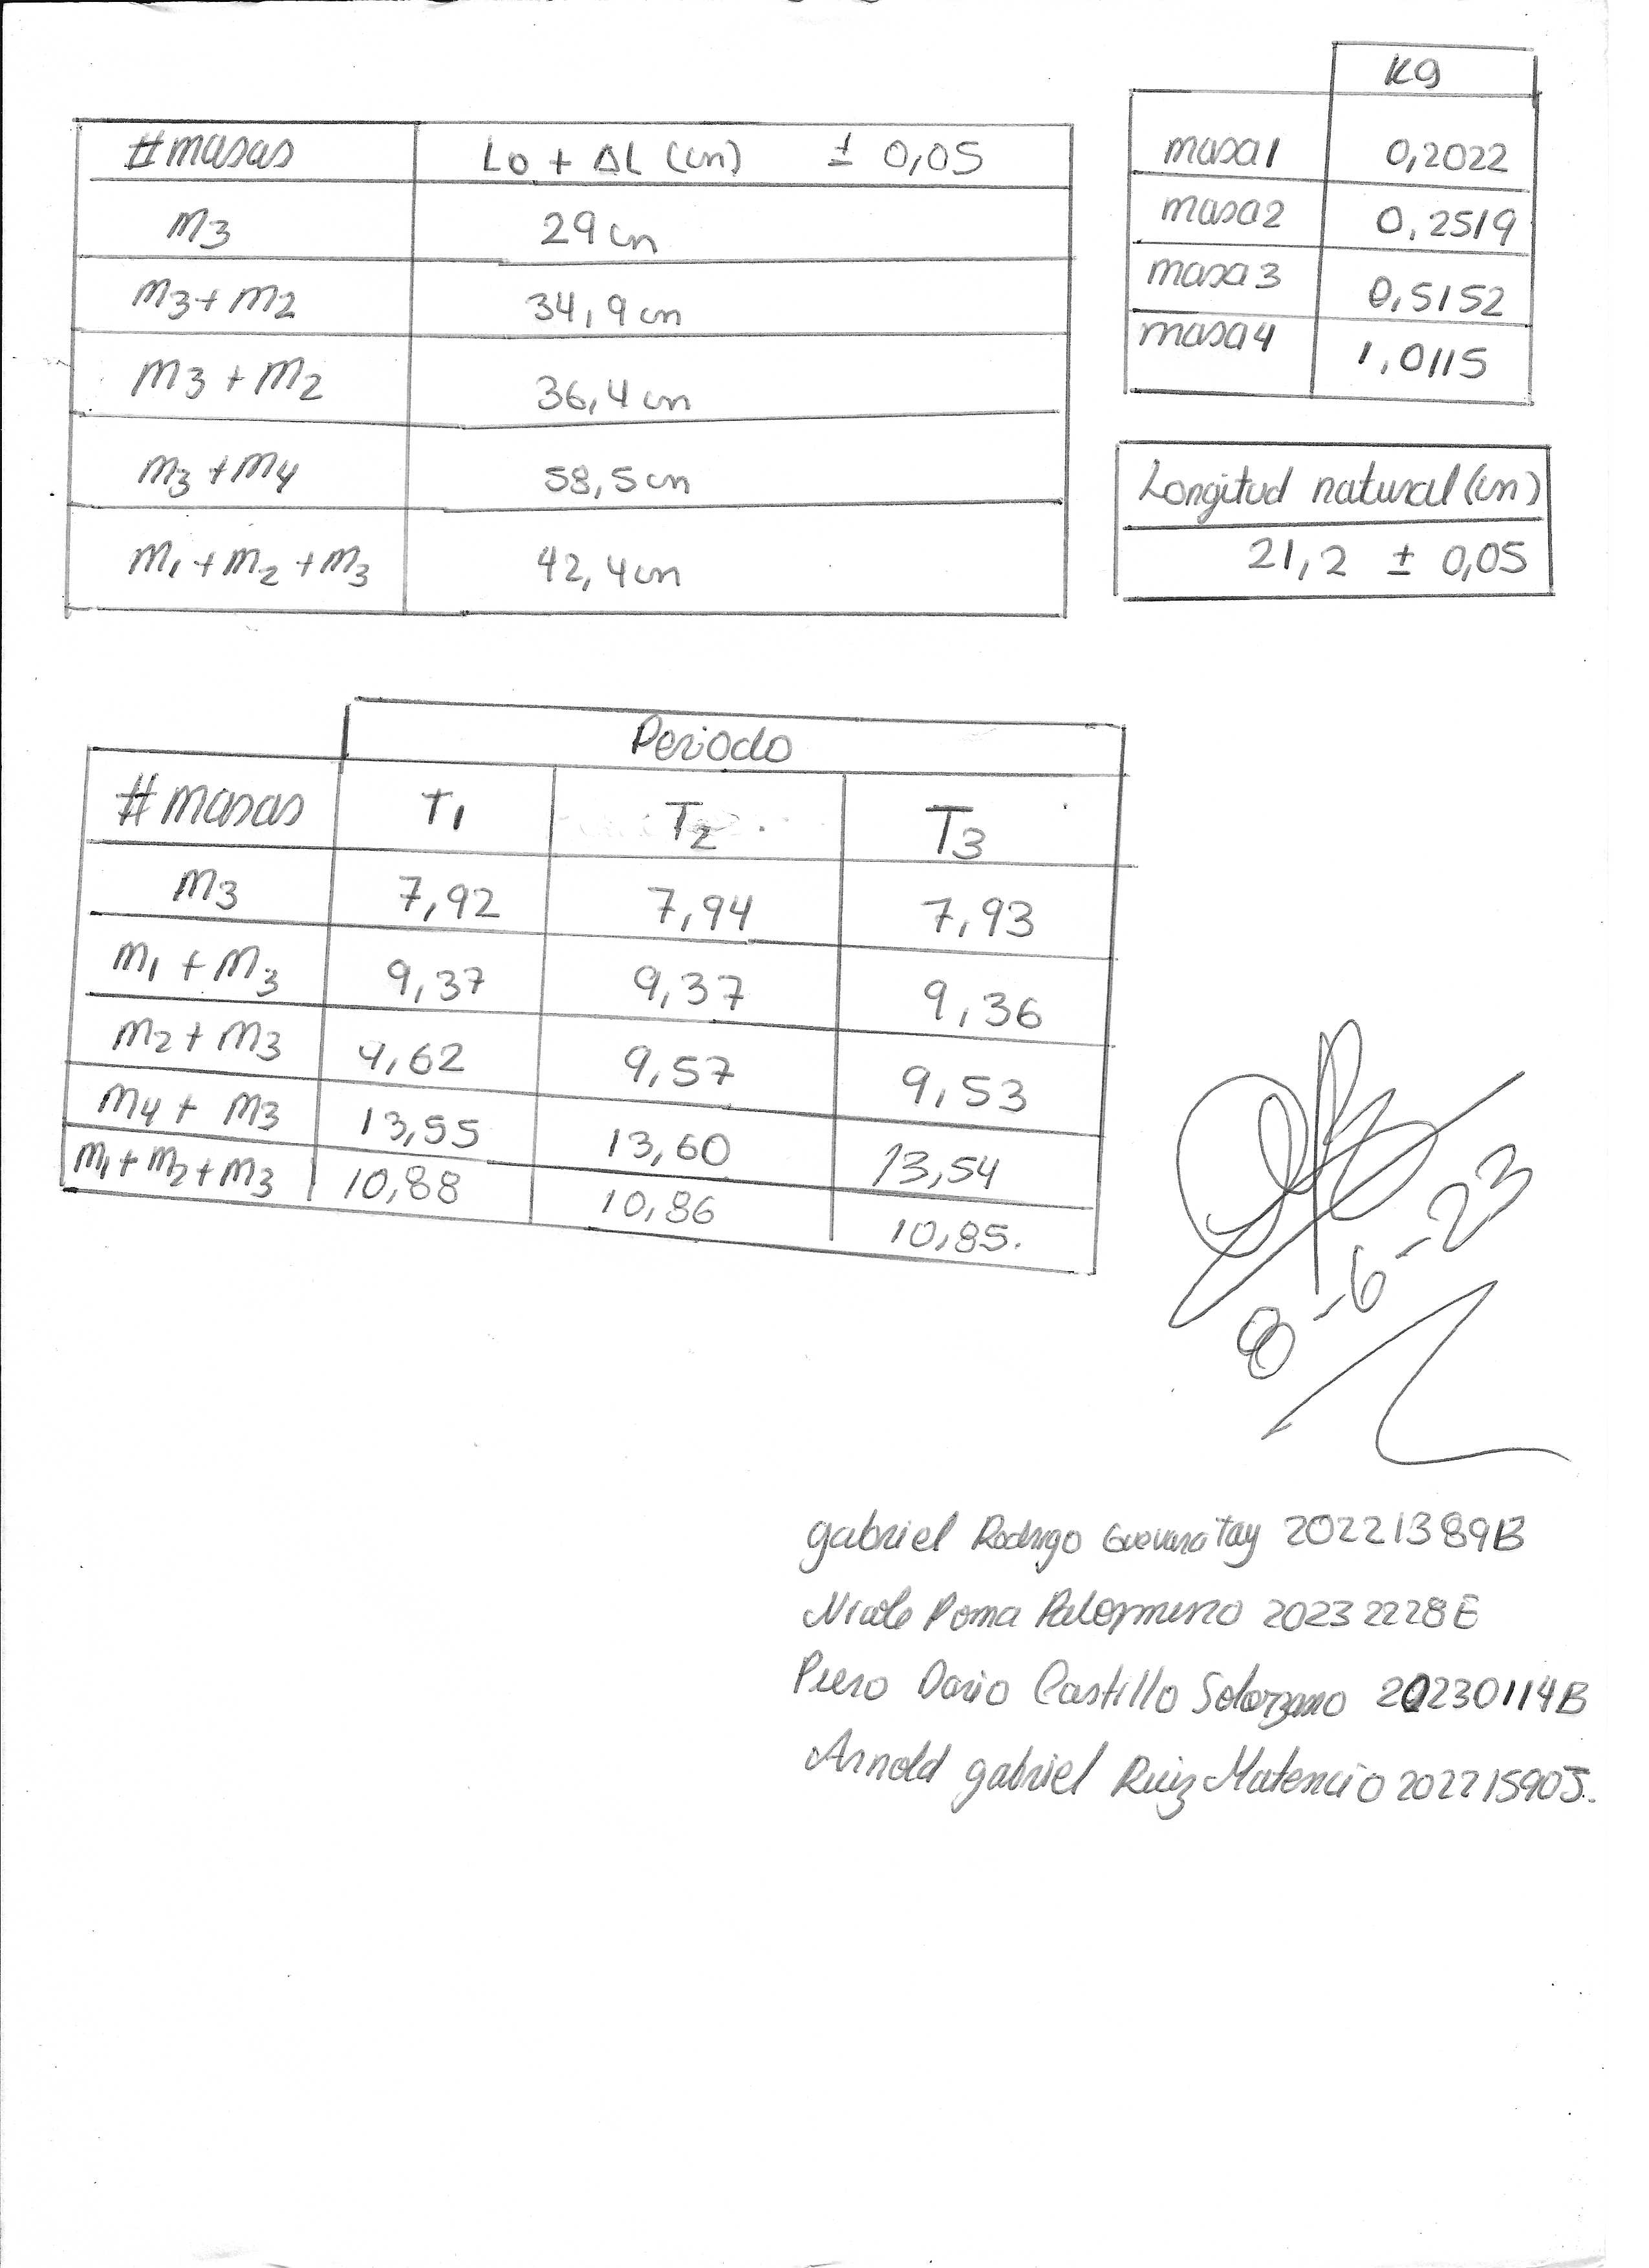
\includegraphics[width=0.8\textwidth]{resources/anexo.png}
    \label{img:annex}
    \caption{Hoja de datos experimentales}
\end{figure}
\end{document}
